\documentclass{beamer}

\mode<presentation> {

% The Beamer class comes with a number of default slide themes
% which change the colors and layouts of slides. Below this is a list
% of all the themes, uncomment each in turn to see what they look like.

%\usetheme{default}
%\usetheme{AnnArbor}
%\usetheme{Antibes}
%\usetheme{Bergen}
%\usetheme{Berkeley}
%\usetheme{Berlin}
%\usetheme{Boadilla}
%\usetheme{CambridgeUS}
%\usetheme{Copenhagen}
%\usetheme{Darmstadt}
%\usetheme{Dresden}
%\usetheme{Frankfurt}
%\usetheme{Goettingen}
%\usetheme{Hannover}
%\usetheme{Ilmenau}
%\usetheme{JuanLesPins}
%\usetheme{Luebeck}
\usetheme{Madrid}
%\usetheme{Malmoe}
%\usetheme{Marburg}
%\usetheme{Montpellier}
%\usetheme{PaloAlto}
%\usetheme{Pittsburgh}
%\usetheme{Rochester}
%\usetheme{Singapore}
%\usetheme{Szeged}
%\usetheme{Warsaw}

% As well as themes, the Beamer class has a number of color themes
% for any slide theme. Uncomment each of these in turn to see how it
% changes the colors of your current slide theme.

%\usecolortheme{albatross}
%\usecolortheme{beaver}
%\usecolortheme{beetle}
%\usecolortheme{crane}
%\usecolortheme{dolphin}
%\usecolortheme{dove}
%\usecolortheme{fly}
%\usecolortheme{lily}
%\usecolortheme{orchid}
%\usecolortheme{rose}
%\usecolortheme{seagull}
%\usecolortheme{seahorse}
%\usecolortheme{whale}
%\usecolortheme{wolverine}

%\setbeamertemplate{footline} % To remove the footer line in all slides uncomment this line
%\setbeamertemplate{footline}[page number] % To replace the footer line in all slides with a simple slide count uncomment this line

%\setbeamertemplate{navigation symbols}{} % To remove the navigation symbols from the bottom of all slides uncomment this line
}


\usepackage[utf8]{inputenc}
\usepackage[english]{babel}
\usepackage{mathtools}
\usepackage{amsmath}
\usepackage{amssymb}
\usepackage{amsfonts}
\usepackage{xcolor}
\usepackage{graphicx}
\usepackage{float}
\usepackage{algorithm}
\usepackage[noend]{algpseudocode}

\let\oldReturn\Return
\renewcommand{\Return}{\State\oldReturn}

\usepackage{pgfplots}
\pgfplotsset{compat=1.15}
\usepackage{tikz}
\usetikzlibrary{arrows,decorations.pathmorphing,positioning,decorations.markings,fit,trees,shapes,automata,shapes.multipart}
\usepackage{pgf-umlsd}
\usepgflibrary{arrows} % for pgf-umlsd

\usepackage{IEEEtrantools}
\usepackage[nomessages]{fp}% http://ctan.org/pkg/fp
\usepackage{listings}

\title[Non-Monotonic Bounds]
      {Non-Monotonic Bounds for Complexity Analysis of Integer Programs}

\author{Fabian B\"{o}ller}

\institute[] {
  RWTH Aachen \\
  \medskip
  \textit{fabian.boeller@rwth-aachen.de}
}

\date{WS 2017/18}

\tikzset{
  transition/.style={align=left,draw},
  location/.style={circle,draw,font=\sffamily\bfseries},
  above tlabel/.style={above right=-0.5cm and 0.2cm},
  transitions/.style={
    every edge/.style={transition},
    every node/.style={font=\sffamily\small}
  },
  scc edge/.style={very thick},
  program/.style={
    ->,>=stealth',auto,node distance=3cm,thick,
    every node/.style={location}
  },
  rvg/.style={
    ->,>=stealth',auto,node distance=1.5cm
  },
  evaluation/.style={
    ->,>=stealth',auto,node distance=2cm,
    every text node part/.style={align=center},thick,
    every node/.style={draw,rectangle}
  },
  cross/.style={
    decoration={ markings,
      mark=at position .5 with {\draw[-,thick] (-2mm,2mm) -- (2mm,-2mm)node[inner sep=1pt,pos=0.5,auto]{#1};}
    },
    postaction={decorate}
  },
  highlight/.style={
    color=blue
  },
  onslide/.code args={<#1>#2}{
    \only<#1>{\pgfkeysalso{#2}}
  },
  invisible/.style={
    opacity=0
  },
  highlight on/.code args={<#1>}{
    \only<#1>{\pgfkeysalso{highlight}}
  },
  show on/.style={
    alt={#1{}{invisible}}
  },
  alt/.code args={<#1>#2#3}{%
    \alt<#1>{\pgfkeysalso{#2}}{\pgfkeysalso{#3}} % \pgfkeysalso doesn't change the path
  },
}

\pgfplotsset{xticklabel={\tick},scaled x ticks=false}
\pgfplotsset{plot coordinates/math parser=false}


\newcommand{\location}{\ell}
\newcommand{\valuation}{\sigma}
\newcommand{\Valuation}{\Sigma}
\newcommand{\update}{\eta}
\newcommand{\atom}{a}
\newcommand{\guard}{\tau}
\newcommand{\cost}{c}
\newcommand{\complexity}{\emph{complexity}}
\newcommand{\landau}{\mathcal{O}}
\newcommand{\constant}{\emph{constant}}

\newcommand{\ValueSet}{\bar{\mathbb{Z}}}

\newcommand{\abs}[1]{\left|#1\right|}

\newcommand{\LSize}{{\mathcal{S}^\sqcup}}
\newcommand{\USize}{{\mathcal{S}^\sqcap}}
\newcommand{\GSize}{{\mathcal{S}^\square}}
\newcommand{\Size}{{(\LSize, \USize)}}
\newcommand{\UTime}{{\mathcal{R}^\sqcap}}
\newcommand{\UCost}{{\mathcal{C}^\sqcap}}
\newcommand{\LLSB}{{\mathcal{S}^\sqcup_l}}
\newcommand{\ULSB}{{\mathcal{S}^\sqcap_l}}
\newcommand{\GLSB}{{\mathcal{S}^\square_l}}
\newcommand{\LSB}{{(\LLSB, \ULSB)}}

\newcommand{\dpre}[1]{{\tilde{d}^{#1}}}
\newcommand{\pret}{r}
\newcommand{\actt}{s}
\newcommand{\prerv}{\gamma}
\newcommand{\actrv}{\alpha}
\newcommand{\outrv}{\beta}
\newcommand{\prestate}{{\tilde{\valuation}}}
\newcommand{\actstate}{\valuation}
\newcommand{\ustate}{{\valuation^\sqcap}}
\newcommand{\lstate}{{\valuation^\sqcup}}
\newcommand{\prel}{{\tilde{\location}}}
\newcommand{\actl}{\location}

\newcommand{\scale}{\emph{scale}}
\newcommand{\incoming}{\emph{in}}
\newcommand{\start}{\emph{start}}
\newcommand{\sign}{\emph{sign}}
\newcommand{\effect}{\emph{effect}}
\newcommand{\SCC}{C}
\newcommand{\timerank}{\emph{timerank}}
\newcommand{\costrank}{\emph{costrank}}
\newcommand{\rv}{\alpha}
\newcommand{\RV}{\text{RV}}
\newcommand{\BoundSet}{\mathcal{B}}
\newcommand{\Program}{\mathcal{P}}
\newcommand{\AtomSet}{\mathcal{A}}
\newcommand{\ConstraintSet}{\mathcal{C}}
\newcommand{\TSet}{\mathcal{T}}
\newcommand{\tvar}{\lambda}
\newcommand{\VSet}{\mathcal{V}}
\newcommand{\TVSet}{\mathcal{TV}}
\newcommand{\PVSet}{\mathcal{PV}}
\newcommand{\AllVarsSet}{(\PVSet \cup \TVSet)}
\newcommand{\LSet}{\mathcal{L}}
\newcommand{\ScaledSum}{\dot{x}}
\newcommand{\pre}{\emph{pre}}
\newcommand{\actV}{\emph{actV}}
\newcommand{\maxO}[1]{\left\langle #1 \right\rangle}
\newcommand{\maximum}[1]{\max \left\lbrace #1 \right\rbrace}
\newcommand{\minimum}[1]{\min \left\lbrace #1 \right\rbrace}
\newcommand{\braced}[1]{\lbrace #1 \rbrace}

\newcommand{\usub}{\delta^\sqcap}
\newcommand{\lsub}{\delta^\sqcup}

\newcommand{\usubst}[3]{\left\lceil #1 \right\rceil^{#3}_{#2}}
\newcommand{\lsubst}[3]{\left\lfloor #1 \right\rfloor^{#3}_{#2}}

\newcommand{\exacteval}[2]{\left\llbracket #1 \right\rrbracket_{#2}}
\newcommand{\ueval}[3]{\left\lceil #1 \right\rceil^{#3}_{#2}}
\newcommand{\leval}[3]{\left\lfloor #1 \right\rfloor^{#3}_{#2}}

\newcommand{\timecomplexityterm}{
  \sup \braced{ k \in \mathbb{N} \mid \exists \valuation_0, (\location, \valuation): \lstate \leq \valuation_0 \leq \ustate \wedge (\location_0, \valuation_0) \rightarrow^k (\location, \valuation) }
}

\newcommand{\timeboundterm}{
  \sup \braced{ k \in \mathbb{N} \mid \exists \valuation_0, (\location, \valuation): \lstate \leq \valuation_0 \leq \ustate \wedge (\location_0, \valuation_0) (\rightarrow^* \circ \rightarrow_t)^k (\location, \valuation) }
}

\newcommand{\sizeboundterm}{
  \braced{ \valuation(v) \mid \exists \valuation_0, (\location, \valuation): \lstate \leq \valuation_0 \leq \ustate \wedge (\location_0, \valuation_0) (\rightarrow^* \circ \rightarrow_\actt) (\location, \valuation)}
}

\newcommand{\usizeboundterm}{\sup \sizeboundterm}
\newcommand{\lsizeboundterm}{\inf \sizeboundterm}

\newcommand{\localsizeboundterm}{
  \braced{\valuation'(v) \mid \exists (\location, \valuation), (\location', \valuation'): \lstate \leq \valuation \leq \ustate \wedge (\location, \valuation) \rightarrow_t (\location', \valuation')}
}

\newcommand{\ulocalsizeboundterm}{\sup \localsizeboundterm}
\newcommand{\llocalsizeboundterm}{\inf \localsizeboundterm}

\newcommand{\costcomplexityterm}{
  \braced{ \sum_{0 \leq i \leq k} \exacteval{\cost(t_i)}{\valuation_i} \mid \exists \valuation_0, k \geq 1: 
    \lstate \leq \valuation_0 \leq \ustate \wedge (\location_0, \valuation_0) \rightarrow_{t_0} (\location_1, \valuation_1) \rightarrow_{t_1} \dots \rightarrow_{t_k} (\location_k, \valuation_k) }
}

\newcommand{\Proof}[2]{
  \input{proofs/#2}
}


\begin{document}

\begin{frame}
  \titlepage % Print the title page as the first slide
\end{frame}

\begin{frame}
\frametitle{Overview} % Table of contents slide, comment this block out to remove it
\tableofcontents % Throughout your presentation, if you choose to use \section{} and \subsection{} commands, these will automatically be printed on this slide as an overview of your presentation
\end{frame}

\section{Introduction}

\slide{Motivation}{motivation}

\slide{Programs}{programs}

\slide{Time Complexity}{time_complexity}

\slide{Ranking Functions}{ranking_functions}

\slide{Time Bounds}{time_bounds}

\slide{Size Bounds}{upper_lower_1}

\slide{Size Bounds}{upper_lower_2}

\begin{frame}
  \frametitle{Size Bounds}
  \begin{figure}
    \centering
    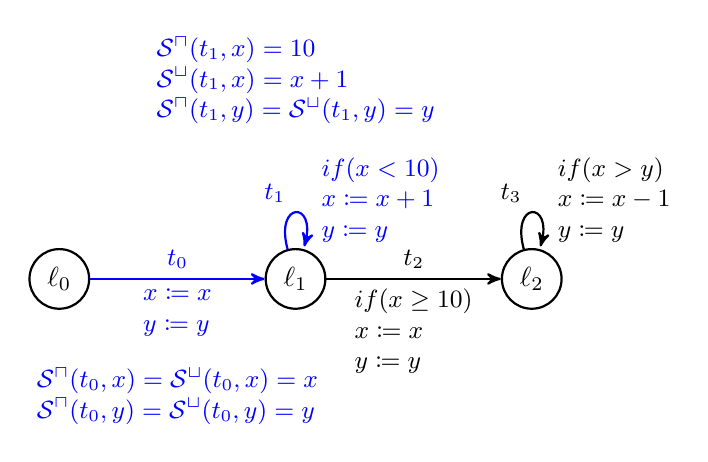
\begin{tikzpicture}[program]
      \node (0) {$\location_0$};
      \node (1) [right of=0] {$\location_1$};
      \node (2) [right of=1] {$\location_2$};
      \path[transitions]
      (0) edge[highlight] node[above] {$t_0$} node[below] {$x \coloneqq x$\\$y \coloneqq y$} node[below=1cm] {$\USize(t_0,x) = \LSize(t_0,x) = x$\\$\USize(t_0,y) = \LSize(t_0,y) = y$} (1)
      (1) edge[highlight, loop above] node[above left] {$t_1$} node[above right=-0.5cm and 0.2cm] {$if(x<10)$\\$x \coloneqq x+1$\\$y \coloneqq y$} node[above=1cm] {$\USize(t_1,x) = 10$\\$\LSize(t_1,x) = x+1$\\$\USize(t_1,y) = \LSize(t_1,y) = y$} (1)
      (1) edge node[above] {$t_2$} node[below] {$if(x \geq 10)$\\$x \coloneqq x$\\$y \coloneqq y$} (2)
      (2) edge[loop above] node[above left] {$t_3$} node[above right=-0.5cm and 0.2cm] {$if(x>y)$\\$x \coloneqq x-1$\\$y \coloneqq y$} (2)
      ;
    \end{tikzpicture}
  \end{figure}
\end{frame}

\begin{frame}
  \frametitle{Size Bounds}
  \begin{figure}
    \centering
    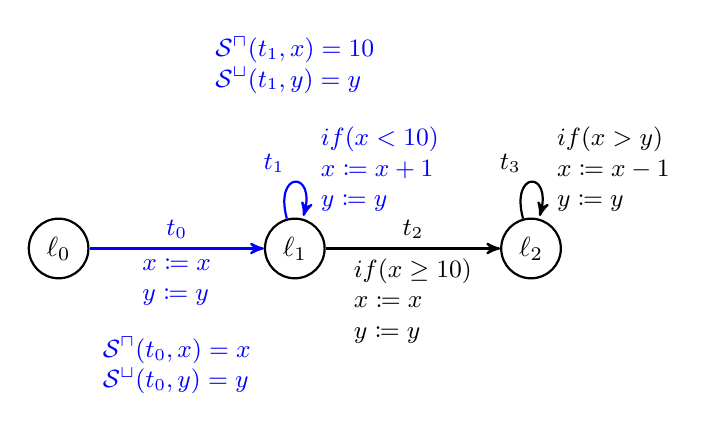
\begin{tikzpicture}[program]
      \node (0) {$\location_0$};
      \node (1) [right of=0] {$\location_1$};
      \node (2) [right of=1] {$\location_2$};
      \path[transitions]
      (0) edge[highlight] node[above] {$t_0$} node[below] {$x \coloneqq x$\\$y \coloneqq y$} node[below=1cm] {$\USize(t_0,x) = x$\\$\LSize(t_0,y) = y$} (1)
      (1) edge[highlight, loop above] node[above left] {$t_1$} node[above right=-0.5cm and 0.2cm] {$if(x<10)$\\$x \coloneqq x+1$\\$y \coloneqq y$} node[above=1cm] {$\USize(t_1,x) = 10$\\$\LSize(t_1,y) = y$} (1)
      (1) edge node[above] {$t_2$} node[below] {$if(x \geq 10)$\\$x \coloneqq x$\\$y \coloneqq y$} (2)
      (2) edge[loop above] node[above left] {$t_3$} node[above right=-0.5cm and 0.2cm] {$if(x>y)$\\$x \coloneqq x-1$\\$y \coloneqq y$} (2)
      ;
    \end{tikzpicture}
  \end{figure}
  \begin{block}{Equation}
    $\UTime(t_3) = \UTime(t_0) \cdot (\USize(t_0,x)-\LSize(t_0,y)) + \UTime(t_1) \cdot (\USize(t_1,x)-\LSize(t_1,y))$ \\
    $\UTime(t_3) = \UTime(t_0) \cdot (x-y) + \UTime(t_1) \cdot (10-y)$
  \end{block}
\end{frame}

\begin{frame}
  \frametitle{Local Size Bounds}
  Define local size bounds
\end{frame}

\begin{frame}
  \frametitle{Time Bounds}
  Back to the example
\end{frame}

\slide{Additive loop}{additive_loop}

\slide{Exponential bounds}{exp_with_scale}

\slide{Exponential bounds}{exp_with_vars}

\begin{frame}
  \frametitle{Size Bounds Caveat}
  Explain size bounds caveat of negating SCCs
\end{frame}

\section{Cost Bounds}

\begin{frame}
  \frametitle{Cost Complexity}
  \begin{block}{Time Complexity}
    TODO Recap
  \end{block}
  \pause
  \begin{block}{Size Complexity}
    TODO Recap
  \end{block}
  \pause
  \begin{block}{Cost Complexity}
    Explain with a call to a function $f$ in the initial example 
  \end{block}
\end{frame}

\begin{frame}
  \frametitle{Cost Complexity}
  Present the trivial approach of multiplying with the time bounds
\end{frame}

\begin{frame}
  \frametitle{Cost Ranking}
\end{frame}

\section{Conclusion}

\begin{frame}
  \frametitle{Conclusion}
\end{frame}

\end{document} 
